\documentclass[11pt,UTF8]{ctexart}
\usepackage{titling}
\usepackage{enumerate}
\usepackage{amsmath}
\usepackage{amssymb}
\usepackage{amsfonts}
\usepackage{listings}
\usepackage{forest}
\usepackage{bm}
\usepackage{float}
\usepackage{graphicx}
\usepackage{multicol}
\usepackage{multirow}
\usepackage{bigstrut}
%\usepackage{booktabs}
\usepackage[unicode=true,%本行非常重要 支持中文目录hyperref CJKbookmarks对二级目录没用
	colorlinks,
	linkcolor=black,
	anchorcolor=black,
	citecolor=black,
	CJKbookmarks=false]{hyperref}
\usepackage{xcolor}
\usepackage{geometry}
\geometry{top=20mm,bottom=20mm,left=20mm,right=20mm}
\pagestyle{plain}%删除页眉
\CTEXsetup[format={\Large\bfseries}]{section}

\def\toprule{\hline}
\def\midrule{\hline}
\def\bottomrule{\hline}

\setlength{\droptitle}{-50pt}%减少标题与页眉距离

\title{数电实验3报告}
\author{17341015\quad数据科学与计算机学院\\计科一班\quad陈鸿峥}
\date{}

\begin{document}
\maketitle
\vspace{-50pt}%减少标题与正文距离

\lstset{language=C++,escapechar=`}

\section{预习报告}
\par 设计一个代码转换电路,输入为4位8421码输出为4位循环码
\subsection{逻辑真值表}
% Table generated by Excel2LaTeX from sheet 'Sheet1'
\begin{table}[htbp]
  \centering
    \begin{tabular}{|r|r|r|r|r|r|r|r|}
    \toprule
    \multicolumn{4}{|c|}{8421码}   & \multicolumn{4}{c|}{4位循环码} \\
    \midrule
    \multicolumn{1}{|p{4.19em}|}{Q3 } & \multicolumn{1}{p{4.19em}|}{Q2 } & \multicolumn{1}{p{4.19em}|}{Q1 } & \multicolumn{1}{p{4.19em}|}{Q0 } & \multicolumn{1}{p{4.19em}|}{G3 } & \multicolumn{1}{p{4.19em}|}{G2 } & \multicolumn{1}{p{4.19em}|}{G1 } & \multicolumn{1}{p{4.19em}|}{G0} \\
    \midrule
    0     & 0     & 0     & 0     & 0     & 0     & 0     & 0 \\
    \midrule
    0     & 0     & 0     & 1     & 0     & 0     & 0     & \textcolor[rgb]{ 1,  0,  0}{1} \\
    \midrule
    0     & 0     & 1     & 0     & 0     & 0     & \textcolor[rgb]{ 1,  0,  0}{1} & \textcolor[rgb]{ 1,  0,  0}{1} \\
    \midrule
    0     & 0     & 1     & 1     & 0     & 0     & \textcolor[rgb]{ 1,  0,  0}{1} & 0 \\
    \midrule
    0     & 1     & 0     & 0     & 0     & \textcolor[rgb]{ 1,  0,  0}{1} & \textcolor[rgb]{ 1,  0,  0}{1} & 0 \\
    \midrule
    0     & 1     & 0     & 1     & 0     & \textcolor[rgb]{ 1,  0,  0}{1} & \textcolor[rgb]{ 1,  0,  0}{1} & \textcolor[rgb]{ 1,  0,  0}{1} \\
    \midrule
    0     & 1     & 1     & 0     & 0     & \textcolor[rgb]{ 1,  0,  0}{1} & 0     & \textcolor[rgb]{ 1,  0,  0}{1} \\
    \midrule
    0     & 1     & 1     & 1     & 0     & \textcolor[rgb]{ 1,  0,  0}{1} & 0     & 0 \\
    \midrule
    1     & 0     & 0     & 0     & \textcolor[rgb]{ 1,  0,  0}{1} & \textcolor[rgb]{ 1,  0,  0}{1} & 0     & 0 \\
    \midrule
    1     & 0     & 0     & 1     & \textcolor[rgb]{ 1,  0,  0}{1} & \textcolor[rgb]{ 1,  0,  0}{1} & 0     & \textcolor[rgb]{ 1,  0,  0}{1} \\
    \midrule
    1     & 0     & 1     & 0     & \textcolor[rgb]{ 1,  0,  0}{1} & \textcolor[rgb]{ 1,  0,  0}{1} & \textcolor[rgb]{ 1,  0,  0}{1} & \textcolor[rgb]{ 1,  0,  0}{1} \\
    \midrule
    1     & 0     & 1     & 1     & \textcolor[rgb]{ 1,  0,  0}{1} & \textcolor[rgb]{ 1,  0,  0}{1} & \textcolor[rgb]{ 1,  0,  0}{1} & 0 \\
    \midrule
    1     & 1     & 0     & 0     & \textcolor[rgb]{ 1,  0,  0}{1} & 0     & \textcolor[rgb]{ 1,  0,  0}{1} & 0 \\
    \midrule
    1     & 1     & 0     & 1     & \textcolor[rgb]{ 1,  0,  0}{1} & 0     & \textcolor[rgb]{ 1,  0,  0}{1} & \textcolor[rgb]{ 1,  0,  0}{1} \\
    \midrule
    1     & 1     & 1     & 0     & \textcolor[rgb]{ 1,  0,  0}{1} & 0     & 0     & \textcolor[rgb]{ 1,  0,  0}{1} \\
    \midrule
    1     & 1     & 1     & 1     & \textcolor[rgb]{ 1,  0,  0}{1} & 0     & 0     & 0 \\
    \bottomrule
    \end{tabular}%
  \label{tab:addlabel}%
\end{table}%


\subsection{设计流程}
由二进制转换为循环码的规则可得
\[G3=Q3,G2=Q3\oplus Q2,G1=Q2\oplus Q1,G0=Q1\oplus Q0\]
\par 设计电路如下:
\begin{figure}[H]
\centering
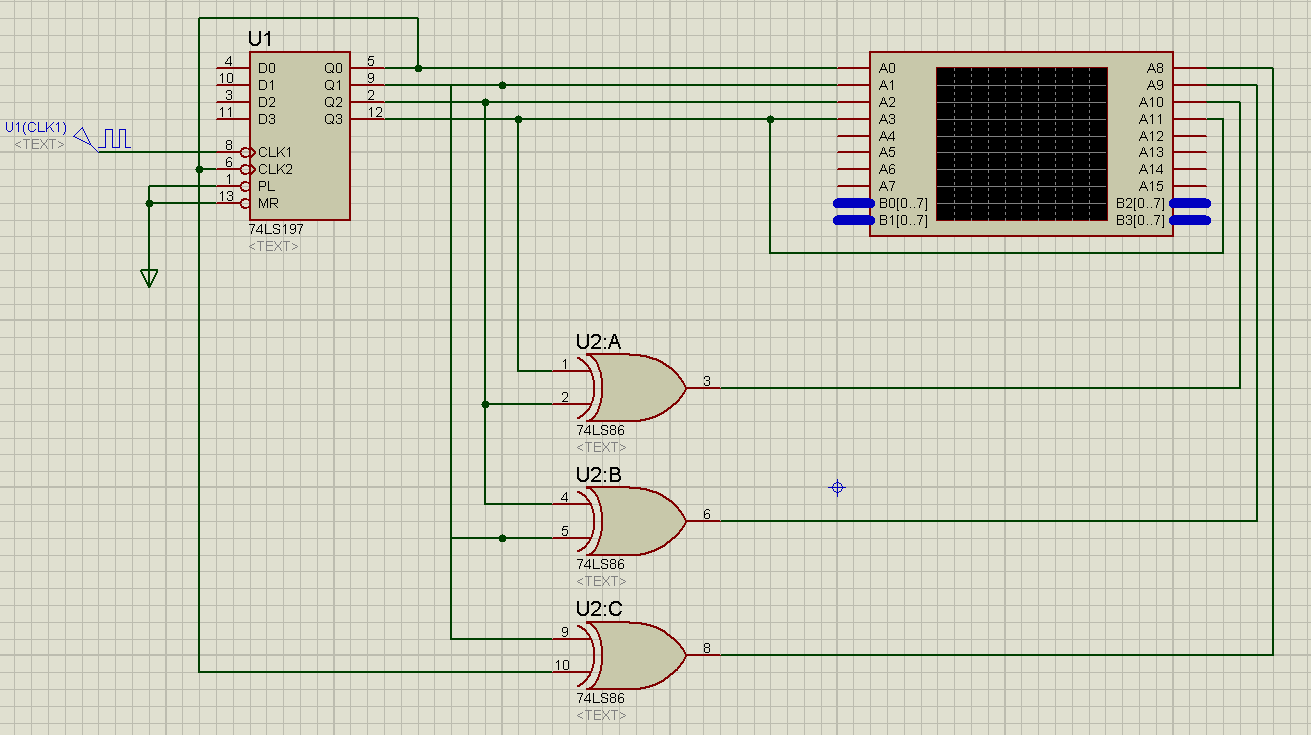
\includegraphics[width=\linewidth]{fig/lab3main.PNG}
\label{Fig:main}
\end{figure}
\par 仿真结果如下:
\begin{figure}[H]
\centering
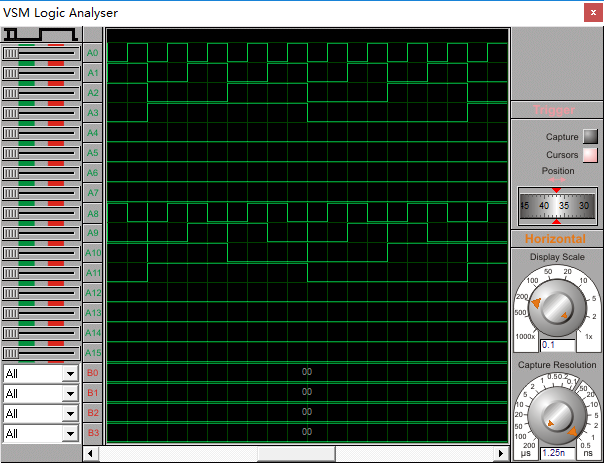
\includegraphics[width=0.8\linewidth]{fig/VSM1.PNG}
\label{Fig:main}
\end{figure}
\par 其中$A0$-$A3$对应$Q0$-$Q3$脚,$A8$-$A11$对应输出$G0$-$G3$脚;连续脉冲频率为$10$Hz. 可见$Q0$-$Q3$输入电平对应$0$-$15$时,$G0$-$G3$输出电平对应其循环码.


\section{加分项目(已在实验课上记录)}
输出16进制数码
\subsection{法一}
直接用逻辑门暴力解决
% Table generated by Excel2LaTeX from sheet 'Sheet1'
\begin{table}[H]
  \centering
    \begin{tabular}{|r|r|r|r|r|r|r|r|r|r|r|r|}
\hline    \multicolumn{1}{|l|}{Q3} & \multicolumn{1}{l|}{Q2} & \multicolumn{1}{l|}{Q1} & \multicolumn{1}{l|}{Q0} & \multicolumn{1}{l|}{NUM} & \multicolumn{1}{l|}{a} & \multicolumn{1}{l|}{b} & \multicolumn{1}{l|}{c} & \multicolumn{1}{l|}{d} & \multicolumn{1}{l|}{e} & \multicolumn{1}{l|}{f} & \multicolumn{1}{l|}{g}   \\
\hline    0     & 0     & 0     & 0     & 0     & \textcolor[rgb]{ 1,  0,  0}{1} & \textcolor[rgb]{ 1,  0,  0}{1} & \textcolor[rgb]{ 1,  0,  0}{1} & \textcolor[rgb]{ 1,  0,  0}{1} & \textcolor[rgb]{ 1,  0,  0}{1} & \textcolor[rgb]{ 1,  0,  0}{1} & 0    \\
\hline    0     & 0     & 0     & 1     & 1     & 0     & \textcolor[rgb]{ 1,  0,  0}{1} & \textcolor[rgb]{ 1,  0,  0}{1} & 0     & 0     & 0     & 0    \\
\hline    0     & 0     & 1     & 0     & 2     & \textcolor[rgb]{ 1,  0,  0}{1} & \textcolor[rgb]{ 1,  0,  0}{1} & 0     & \textcolor[rgb]{ 1,  0,  0}{1} & \textcolor[rgb]{ 1,  0,  0}{1} & 0     & \textcolor[rgb]{ 1,  0,  0}{1} \\
\hline    0     & 0     & 1     & 1     & 3     & \textcolor[rgb]{ 1,  0,  0}{1} & \textcolor[rgb]{ 1,  0,  0}{1} & \textcolor[rgb]{ 1,  0,  0}{1} & \textcolor[rgb]{ 1,  0,  0}{1} & 0     & 0     & \textcolor[rgb]{ 1,  0,  0}{1}  \\
\hline    0     & 1     & 0     & 0     & 4     & 0     & \textcolor[rgb]{ 1,  0,  0}{1} & \textcolor[rgb]{ 1,  0,  0}{1} & 0     & 0     & \textcolor[rgb]{ 1,  0,  0}{1} & \textcolor[rgb]{ 1,  0,  0}{1}   \\
\hline    0     & 1     & 0     & 1     & 5     & \textcolor[rgb]{ 1,  0,  0}{1} & 0     & \textcolor[rgb]{ 1,  0,  0}{1} & \textcolor[rgb]{ 1,  0,  0}{1} & 0     & \textcolor[rgb]{ 1,  0,  0}{1} & \textcolor[rgb]{ 1,  0,  0}{1}   \\
\hline    0     & 1     & 1     & 0     & 6     & \textcolor[rgb]{ 1,  0,  0}{1} & 0     & \textcolor[rgb]{ 1,  0,  0}{1} & \textcolor[rgb]{ 1,  0,  0}{1} & \textcolor[rgb]{ 1,  0,  0}{1} & \textcolor[rgb]{ 1,  0,  0}{1} & \textcolor[rgb]{ 1,  0,  0}{1}   \\
\hline    0     & 1     & 1     & 1     & 7     & \textcolor[rgb]{ 1,  0,  0}{1} & \textcolor[rgb]{ 1,  0,  0}{1} & \textcolor[rgb]{ 1,  0,  0}{1} & 0     & 0     & 0     & 0       \\
\hline    1     & 0     & 0     & 0     & 8     & \textcolor[rgb]{ 1,  0,  0}{1} & \textcolor[rgb]{ 1,  0,  0}{1} & \textcolor[rgb]{ 1,  0,  0}{1} & \textcolor[rgb]{ 1,  0,  0}{1} & \textcolor[rgb]{ 1,  0,  0}{1} & \textcolor[rgb]{ 1,  0,  0}{1} & \textcolor[rgb]{ 1,  0,  0}{1}   \\
\hline    1     & 0     & 0     & 1     & 9     & \textcolor[rgb]{ 1,  0,  0}{1} & \textcolor[rgb]{ 1,  0,  0}{1} & \textcolor[rgb]{ 1,  0,  0}{1} & \textcolor[rgb]{ 1,  0,  0}{1} & 0     & \textcolor[rgb]{ 1,  0,  0}{1} & \textcolor[rgb]{ 1,  0,  0}{1}   \\
\hline    1     & 0     & 1     & 0     & A     & \textcolor[rgb]{ 1,  0,  0}{1} & \textcolor[rgb]{ 1,  0,  0}{1} & \textcolor[rgb]{ 1,  0,  0}{1} & 0     & \textcolor[rgb]{ 1,  0,  0}{1} & \textcolor[rgb]{ 1,  0,  0}{1} & \textcolor[rgb]{ 1,  0,  0}{1}   \\
\hline    1     & 0     & 1     & 1     & b     & 0     & 0     & \textcolor[rgb]{ 1,  0,  0}{1} & \textcolor[rgb]{ 1,  0,  0}{1} & \textcolor[rgb]{ 1,  0,  0}{1} & \textcolor[rgb]{ 1,  0,  0}{1} & \textcolor[rgb]{ 1,  0,  0}{1}   \\
\hline    1     & 1     & 0     & 0     & C     & \textcolor[rgb]{ 1,  0,  0}{1} & 0     & 0     & \textcolor[rgb]{ 1,  0,  0}{1} & \textcolor[rgb]{ 1,  0,  0}{1} & \textcolor[rgb]{ 1,  0,  0}{1} & 0       \\
\hline    1     & 1     & 0     & 1     & d     & 0     & \textcolor[rgb]{ 1,  0,  0}{1} & \textcolor[rgb]{ 1,  0,  0}{1} & \textcolor[rgb]{ 1,  0,  0}{1} & \textcolor[rgb]{ 1,  0,  0}{1} & 0     & \textcolor[rgb]{ 1,  0,  0}{1}   \\
\hline    1     & 1     & 1     & 0     & E     & \textcolor[rgb]{ 1,  0,  0}{1} & 0     & 0     & \textcolor[rgb]{ 1,  0,  0}{1} & \textcolor[rgb]{ 1,  0,  0}{1} & \textcolor[rgb]{ 1,  0,  0}{1} & \textcolor[rgb]{ 1,  0,  0}{1}   \\
\hline    1     & 1     & 1     & 1     & F     & \textcolor[rgb]{ 1,  0,  0}{1} & 0     & 0     & 0     & \textcolor[rgb]{ 1,  0,  0}{1} & \textcolor[rgb]{ 1,  0,  0}{1} & \textcolor[rgb]{ 1,  0,  0}{1}   \\
\hline    \end{tabular}%
  \label{tab:addlabel}%
\end{table}%
\par 设$G3$为$A$,$G2$为$B$,$G1$为$C$,$G0$为$D$,用POS形式表示有
\[\begin{aligned}
a&=M_{3,5,12,15}\\
b&=M_{1,2,4,5,10,11}\\
c&=M_{1,2,4,14}\\
d&=M_{1,6,9,12,15}\\
e&=M_{7,9,11,12,13,15}\\
f&=M_{3,9,13,14,15}\\
g&=M_{4,9,15,16}
\end{aligned}\]
\par 设计电路如下图所示
\begin{figure}[H]
\centering
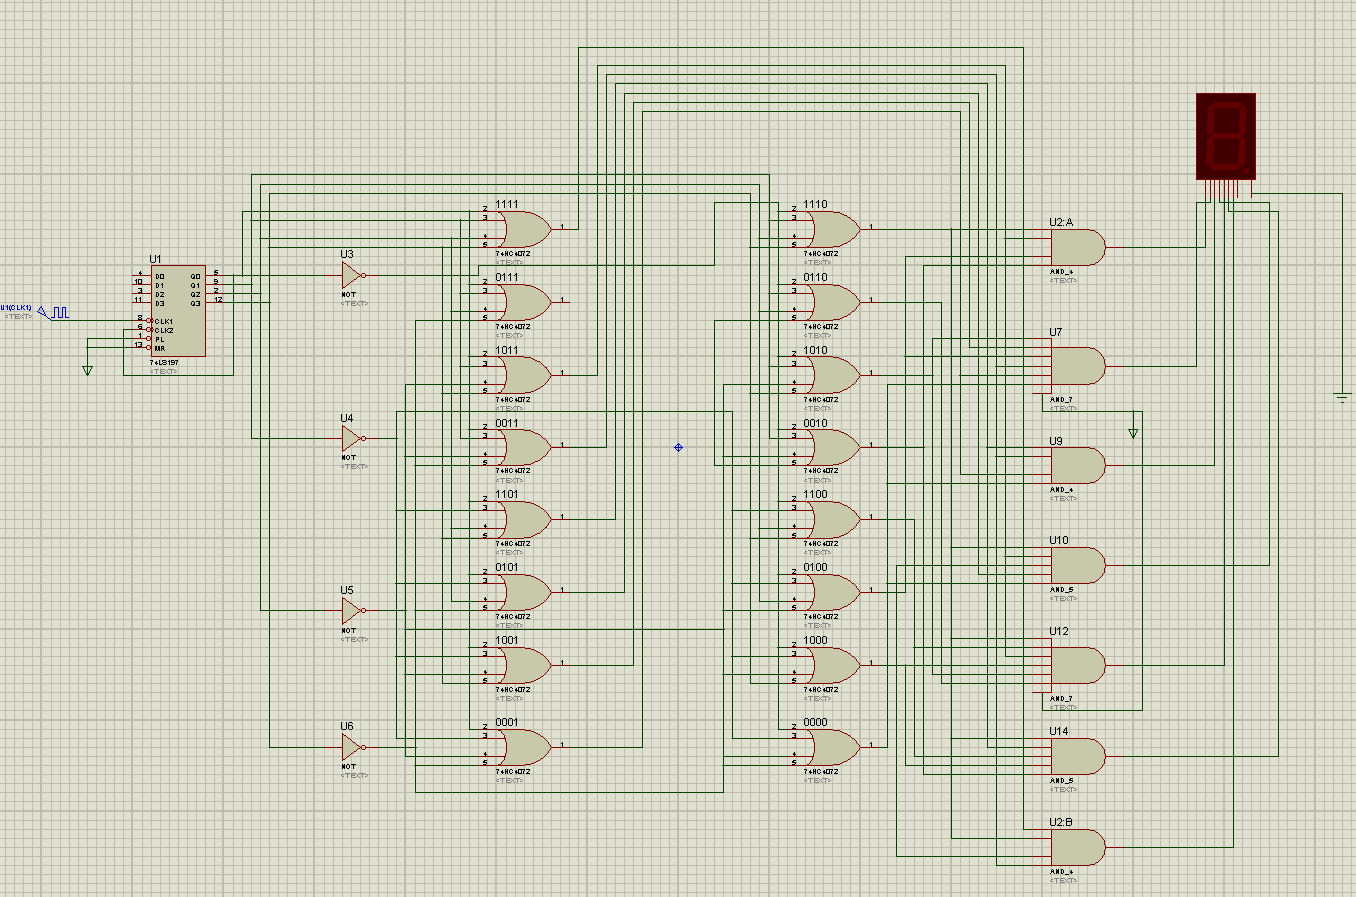
\includegraphics[width=\linewidth]{fig/lab3_plus.PNG}
\label{Fig:plus}
\end{figure}
\par 左边是将所有$M_i$均列出来,右侧再进行整合

\subsection{法二}
采用选择器(MUX)构造,这里选用的是74HC151,比较起法一会简单得多. Q1、Q2、Q3作为MUX的A、B、C输入,通过比较输出与Q0的异同,可通过恰当连线使得MUX表示任意四元逻辑表达式. 下面的真值表列出了构造,其中N代表$\overline{Q0}$(Q0取非),S代表$Q0$(与Q0)相同,$1$代表输出恒为$1$(接电源),$0$代表输出恒为$0$(接地).
% Table generated by Excel2LaTeX from sheet 'Sheet2'
\begin{table}[H]
  \centering
    \begin{tabular}{|r|r|r|r|r|c|r|c|r|c|r|c|r|c|r|c|r|c|}
    \hline
    \multicolumn{1}{|l|}{Q3} & \multicolumn{1}{l|}{Q2} & \multicolumn{1}{l|}{Q1} & \multicolumn{1}{l|}{Q0} & \multicolumn{2}{c|}{a} & \multicolumn{2}{c|}{b} & \multicolumn{2}{c|}{c} & \multicolumn{2}{c|}{d} & \multicolumn{2}{c|}{e} & \multicolumn{2}{c|}{f} & \multicolumn{2}{c|}{g} \bigstrut\\
    \hline
    0     & 0     & 0     & 0     & \textcolor[rgb]{ 1,  0,  0}{1} & \multirow{2}[4]{*}{N} & \textcolor[rgb]{ 1,  0,  0}{1} & \multirow{2}[4]{*}{1} & \textcolor[rgb]{ 1,  0,  0}{1} & \multirow{2}[4]{*}{1} & \textcolor[rgb]{ 1,  0,  0}{1} & \multirow{2}[4]{*}{N} & \textcolor[rgb]{ 1,  0,  0}{1} & \multirow{2}[4]{*}{N} & \textcolor[rgb]{ 1,  0,  0}{1} & \multirow{2}[4]{*}{N} & 0     & \multirow{2}[4]{*}{0} \bigstrut\\
\cline{1-5}\cline{7-7}\cline{9-9}\cline{11-11}\cline{13-13}\cline{15-15}\cline{17-17}    0     & 0     & 0     & 1     & 0     &       & \textcolor[rgb]{ 1,  0,  0}{1} &       & \textcolor[rgb]{ 1,  0,  0}{1} &       & 0     &       & 0     &       & 0     &       & 0     &  \bigstrut\\
    \hline
    0     & 0     & 1     & 0     & \textcolor[rgb]{ 1,  0,  0}{1} & \multirow{2}[4]{*}{1} & \textcolor[rgb]{ 1,  0,  0}{1} & \multirow{2}[4]{*}{1} & 0     & \multirow{2}[4]{*}{S} & \textcolor[rgb]{ 1,  0,  0}{1} & \multirow{2}[4]{*}{1} & \textcolor[rgb]{ 1,  0,  0}{1} & \multirow{2}[4]{*}{N} & 0     & \multirow{2}[4]{*}{0} & \textcolor[rgb]{ 1,  0,  0}{1} & \multirow{2}[4]{*}{1} \bigstrut\\
\cline{1-5}\cline{7-7}\cline{9-9}\cline{11-11}\cline{13-13}\cline{15-15}\cline{17-17}    0     & 0     & 1     & 1     & \textcolor[rgb]{ 1,  0,  0}{1} &       & \textcolor[rgb]{ 1,  0,  0}{1} &       & \textcolor[rgb]{ 1,  0,  0}{1} &       & \textcolor[rgb]{ 1,  0,  0}{1} &       & 0     &       & 0     &       & \textcolor[rgb]{ 1,  0,  0}{1} &  \bigstrut\\
    \hline
    0     & 1     & 0     & 0     & 0     & \multirow{2}[4]{*}{S} & \textcolor[rgb]{ 1,  0,  0}{1} & \multirow{2}[4]{*}{N} & \textcolor[rgb]{ 1,  0,  0}{1} & \multirow{2}[4]{*}{1} & 0     & \multirow{2}[4]{*}{S} & 0     & \multirow{2}[4]{*}{0} & \textcolor[rgb]{ 1,  0,  0}{1} & \multirow{2}[4]{*}{1} & \textcolor[rgb]{ 1,  0,  0}{1} & \multirow{2}[4]{*}{1} \bigstrut\\
\cline{1-5}\cline{7-7}\cline{9-9}\cline{11-11}\cline{13-13}\cline{15-15}\cline{17-17}    0     & 1     & 0     & 1     & \textcolor[rgb]{ 1,  0,  0}{1} &       & 0     &       & \textcolor[rgb]{ 1,  0,  0}{1} &       & \textcolor[rgb]{ 1,  0,  0}{1} &       & 0     &       & \textcolor[rgb]{ 1,  0,  0}{1} &       & \textcolor[rgb]{ 1,  0,  0}{1} &  \bigstrut\\
    \hline
    0     & 1     & 1     & 0     & \textcolor[rgb]{ 1,  0,  0}{1} & \multirow{2}[4]{*}{1} & 0     & \multirow{2}[4]{*}{S} & \textcolor[rgb]{ 1,  0,  0}{1} & \multirow{2}[4]{*}{1} & \textcolor[rgb]{ 1,  0,  0}{1} & \multirow{2}[4]{*}{N} & \textcolor[rgb]{ 1,  0,  0}{1} & \multirow{2}[4]{*}{N} & \textcolor[rgb]{ 1,  0,  0}{1} & \multirow{2}[4]{*}{N} & \textcolor[rgb]{ 1,  0,  0}{1} & \multirow{2}[4]{*}{N} \bigstrut\\
\cline{1-5}\cline{7-7}\cline{9-9}\cline{11-11}\cline{13-13}\cline{15-15}\cline{17-17}    0     & 1     & 1     & 1     & \textcolor[rgb]{ 1,  0,  0}{1} &       & \textcolor[rgb]{ 1,  0,  0}{1} &       & \textcolor[rgb]{ 1,  0,  0}{1} &       & 0     &       & 0     &       & 0     &       & 0     &  \bigstrut\\
    \hline
    1     & 0     & 0     & 0     & \textcolor[rgb]{ 1,  0,  0}{1} & \multirow{2}[4]{*}{1} & \textcolor[rgb]{ 1,  0,  0}{1} & \multirow{2}[4]{*}{1} & \textcolor[rgb]{ 1,  0,  0}{1} & \multirow{2}[4]{*}{1} & \textcolor[rgb]{ 1,  0,  0}{1} & \multirow{2}[4]{*}{1} & \textcolor[rgb]{ 1,  0,  0}{1} & \multirow{2}[4]{*}{N} & \textcolor[rgb]{ 1,  0,  0}{1} & \multirow{2}[4]{*}{1} & \textcolor[rgb]{ 1,  0,  0}{1} & \multirow{2}[4]{*}{1} \bigstrut\\
\cline{1-5}\cline{7-7}\cline{9-9}\cline{11-11}\cline{13-13}\cline{15-15}\cline{17-17}    1     & 0     & 0     & 1     & \textcolor[rgb]{ 1,  0,  0}{1} &       & \textcolor[rgb]{ 1,  0,  0}{1} &       & \textcolor[rgb]{ 1,  0,  0}{1} &       & \textcolor[rgb]{ 1,  0,  0}{1} &       & 0     &       & \textcolor[rgb]{ 1,  0,  0}{1} &       & \textcolor[rgb]{ 1,  0,  0}{1} &  \bigstrut\\
    \hline
    1     & 0     & 1     & 0     & \textcolor[rgb]{ 1,  0,  0}{1} & \multirow{2}[4]{*}{N} & \textcolor[rgb]{ 1,  0,  0}{1} & \multirow{2}[4]{*}{N} & \textcolor[rgb]{ 1,  0,  0}{1} & \multirow{2}[4]{*}{1} & 0     & \multirow{2}[4]{*}{S} & \textcolor[rgb]{ 1,  0,  0}{1} & \multirow{2}[4]{*}{1} & \textcolor[rgb]{ 1,  0,  0}{1} & \multirow{2}[4]{*}{1} & \textcolor[rgb]{ 1,  0,  0}{1} & \multirow{2}[4]{*}{1} \bigstrut\\
\cline{1-5}\cline{7-7}\cline{9-9}\cline{11-11}\cline{13-13}\cline{15-15}\cline{17-17}    1     & 0     & 1     & 1     & 0     &       & 0     &       & \textcolor[rgb]{ 1,  0,  0}{1} &       & \textcolor[rgb]{ 1,  0,  0}{1} &       & \textcolor[rgb]{ 1,  0,  0}{1} &       & \textcolor[rgb]{ 1,  0,  0}{1} &       & \textcolor[rgb]{ 1,  0,  0}{1} &  \bigstrut\\
    \hline
    1     & 1     & 0     & 0     & \textcolor[rgb]{ 1,  0,  0}{1} & \multirow{2}[4]{*}{N} & 0     & \multirow{2}[4]{*}{S} & 0     & \multirow{2}[4]{*}{S} & \textcolor[rgb]{ 1,  0,  0}{1} & \multirow{2}[4]{*}{1} & \textcolor[rgb]{ 1,  0,  0}{1} & \multirow{2}[4]{*}{1} & \textcolor[rgb]{ 1,  0,  0}{1} & \multirow{2}[4]{*}{N} & 0     & \multirow{2}[4]{*}{S} \bigstrut\\
\cline{1-5}\cline{7-7}\cline{9-9}\cline{11-11}\cline{13-13}\cline{15-15}\cline{17-17}    1     & 1     & 0     & 1     & 0     &       & \textcolor[rgb]{ 1,  0,  0}{1} &       & \textcolor[rgb]{ 1,  0,  0}{1} &       & \textcolor[rgb]{ 1,  0,  0}{1} &       & \textcolor[rgb]{ 1,  0,  0}{1} &       & 0     &       & \textcolor[rgb]{ 1,  0,  0}{1} &  \bigstrut\\
    \hline
    1     & 1     & 1     & 0     & \textcolor[rgb]{ 1,  0,  0}{1} & \multirow{2}[4]{*}{1} & 0     & \multirow{2}[4]{*}{0} & 0     & \multirow{2}[4]{*}{0} & \textcolor[rgb]{ 1,  0,  0}{1} & \multirow{2}[4]{*}{N} & \textcolor[rgb]{ 1,  0,  0}{1} & \multirow{2}[4]{*}{1} & \textcolor[rgb]{ 1,  0,  0}{1} & \multirow{2}[4]{*}{1} & \textcolor[rgb]{ 1,  0,  0}{1} & \multirow{2}[4]{*}{1} \bigstrut\\
\cline{1-5}\cline{7-7}\cline{9-9}\cline{11-11}\cline{13-13}\cline{15-15}\cline{17-17}    1     & 1     & 1     & 1     & \textcolor[rgb]{ 1,  0,  0}{1} &       & 0     &       & 0     &       & 0     &       & \textcolor[rgb]{ 1,  0,  0}{1} &       & \textcolor[rgb]{ 1,  0,  0}{1} &       & \textcolor[rgb]{ 1,  0,  0}{1} &  \bigstrut\\
    \hline
    \end{tabular}%
  \label{tab:addlabel}%
\end{table}%
\par 实验电路如下
\begin{figure}[H]
\centering
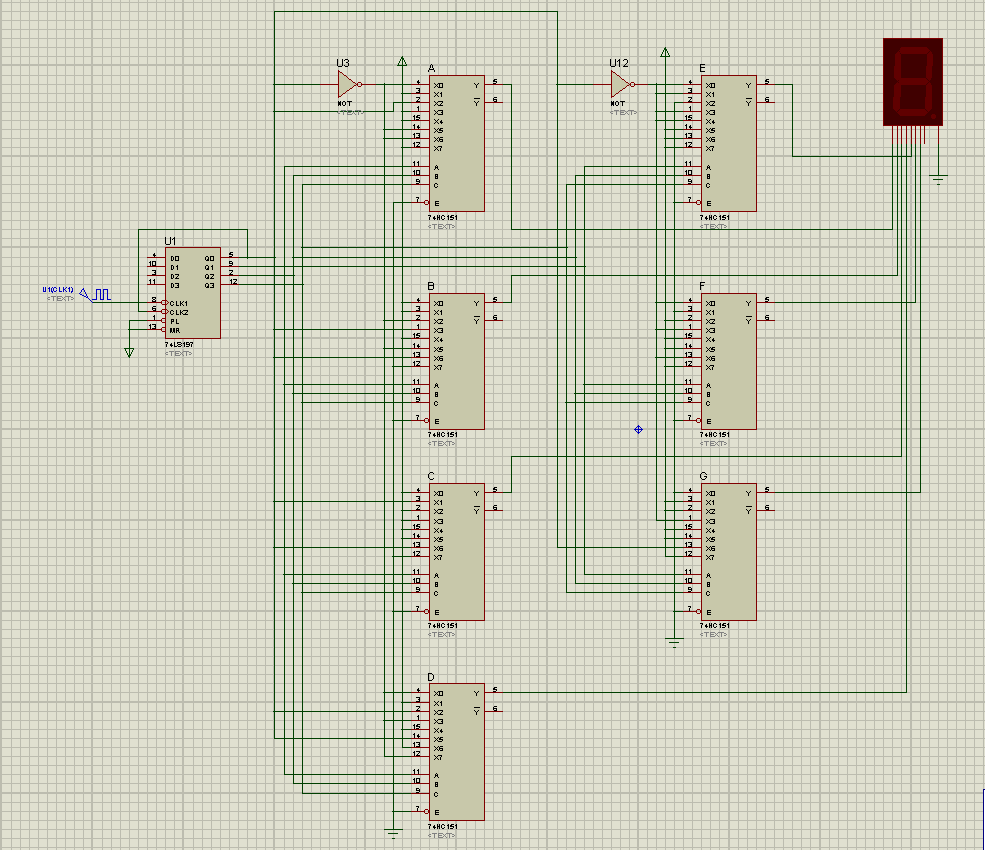
\includegraphics[width=\linewidth]{fig/lab3plus2.PNG}
\label{Fig:plus2}
\end{figure}
\par 经测试可得出正确结果



\section{实验报告}
\subsection{实验仪器及器件}
\begin{enumerate}
    \item 数字电路实验箱、示波器
    \item 74LS197*1、74LS86*1
\end{enumerate}

\subsection{实验箱静态、动态测试步骤}
\begin{enumerate}
    \item 接通实验箱电源
    \item 用逻辑开关模拟二进制代码输入,并把输出接入“0-1”显示器(即实验箱有右上角LED灯);检查电路,看电路是否正常操作
    \item 用74LS197构成十六进制计数器作为代码转换电路的输入信号源,其中CP0作为时钟输入(接连续脉冲或单步脉冲),QO与CP1相连,$\overline{MR}$、$\overline{PL}$接HIGH,Q3、Q2、Q1、Q0为十六进制计数器的输出
    \item 按照预习报告的电路图连接74LS197和74LS86
    \item 将74LS86的输出连接到“0-1”显示器和示波器中,注意示波器两侧的导线要接地
    \item 观察“0-1”显示器的数码变化及示波器的波形变化,进行实验分析
\end{enumerate}

\subsection{结果分析及结论}
\begin{figure}[H]
\centering
\includegraphics[width=\linewidth]{fig/DS2_QuickPrint1.png}
\label{Fig:DS2}
\end{figure}
这里的$D0$-$D3$对应74LS86输出的$Q3$-$Q0$. 从图中可以看出4位循环码的排布;并且,与仿真结果类似,同样出现了毛刺现象(尖峰脉冲),这是因为组合电路中存在着竞争与冒险行为(实验八,还未进行深究,但这是个有意思的问题).


\section{心得体会}
\begin{enumerate}
    \item 学会基本逻辑电路的设计与分析过程
    \item 进一步熟悉Proteus的操作,但是连线实在太麻烦了!!!
    \item 进一步学会调整示波器,使其能够正确稳定显示波形
\end{enumerate}


\end{document}